
%% bare_conf.tex
%% V1.4b
%% 2015/08/26
%% by Michael Shell
%% See:
%% http://www.michaelshell.org/
%% for current contact information.
%%
%% This is a skeleton file demonstrating the use of IEEEtran.cls
%% (requires IEEEtran.cls version 1.8b or later) with an IEEE
%% conference paper.
%%
%% Support sites:
%% http://www.michaelshell.org/tex/ieeetran/
%% http://www.ctan.org/pkg/ieeetran
%% and
%% http://www.ieee.org/

%%*************************************************************************
%% Legal Notice:
%% This code is offered as-is without any warranty either expressed or
%% implied; without even the implied warranty of MERCHANTABILITY or
%% FITNESS FOR A PARTICULAR PURPOSE! 
%% User assumes all risk.
%% In no event shall the IEEE or any contributor to this code be liable for
%% any damages or losses, including, but not limited to, incidental,
%% consequential, or any other damages, resulting from the use or misuse
%% of any information contained here.
%%
%% All comments are the opinions of their respective authors and are not
%% necessarily endorsed by the IEEE.
%%
%% This work is distributed under the LaTeX Project Public License (LPPL)
%% ( http://www.latex-project.org/ ) version 1.3, and may be freely used,
%% distributed and modified. A copy of the LPPL, version 1.3, is included
%% in the base LaTeX documentation of all distributions of LaTeX released
%% 2003/12/01 or later.
%% Retain all contribution notices and credits.
%% ** Modified files should be clearly indicated as such, including  **
%% ** renaming them and changing author support contact information. **
%%*************************************************************************


% *** Authors should verify (and, if needed, correct) their LaTeX system  ***
% *** with the testflow diagnostic prior to trusting their LaTeX platform ***
% *** with production work. The IEEE's font choices and paper sizes can   ***
% *** trigger bugs that do not appear when using other class files.       ***                          ***
% The testflow support page is at:
% http://www.michaelshell.org/tex/testflow/



\documentclass[conference]{IEEEtran}
\usepackage[utf8]{inputenc}
\usepackage{graphicx}
\usepackage{subfigure}
\usepackage{amsmath} % assumes amsmath package installed
\usepackage{amssymb} 
\usepackage{array}

\usepackage{blindtext}
\usepackage{color}

% Some Computer Society conferences also require the compsoc mode option,
% but others use the standard conference format.
%
% If IEEEtran.cls has not been installed into the LaTeX system files,
% manually specify the path to it like:
% \documentclass[conference]{../sty/IEEEtran}





% Some very useful LaTeX packages include:
% (uncomment the ones you want to load)


% *** MISC UTILITY PACKAGES ***
%
%\usepackage{ifpdf}
% Heiko Oberdiek's ifpdf.sty is very useful if you need conditional
% compilation based on whether the output is pdf or dvi.
% usage:
% \ifpdf
%   % pdf code
% \else
%   % dvi code
% \fi
% The latest version of ifpdf.sty can be obtained from:
% http://www.ctan.org/pkg/ifpdf
% Also, note that IEEEtran.cls V1.7 and later provides a builtin
% \ifCLASSINFOpdf conditional that works the same way.
% When switching from latex to pdflatex and vice-versa, the compiler may
% have to be run twice to clear warning/error messages.






% *** CITATION PACKAGES ***
%
%\usepackage{cite}
% cite.sty was written by Donald Arseneau
% V1.6 and later of IEEEtran pre-defines the format of the cite.sty package
% \cite{} output to follow that of the IEEE. Loading the cite package will
% result in citation numbers being automatically sorted and properly
% "compressed/ranged". e.g., [1], [9], [2], [7], [5], [6] without using
% cite.sty will become [1], [2], [5]--[7], [9] using cite.sty. cite.sty's
% \cite will automatically add leading space, if needed. Use cite.sty's
% noadjust option (cite.sty V3.8 and later) if you want to turn this off
% such as if a citation ever needs to be enclosed in parenthesis.
% cite.sty is already installed on most LaTeX systems. Be sure and use
% version 5.0 (2009-03-20) and later if using hyperref.sty.
% The latest version can be obtained at:
% http://www.ctan.org/pkg/cite
% The documentation is contained in the cite.sty file itself.






% *** GRAPHICS RELATED PACKAGES ***
%
\ifCLASSINFOpdf
  % \usepackage[pdftex]{graphicx}
  % declare the path(s) where your graphic files are
  % \graphicspath{{../pdf/}{../jpeg/}}
  % and their extensions so you won't have to specify these with
  % every instance of \includegraphics
  % \DeclareGraphicsExtensions{.pdf,.jpeg,.png}
\else
  % or other class option (dvipsone, dvipdf, if not using dvips). graphicx
  % will default to the driver specified in the system graphics.cfg if no
  % driver is specified.
  % \usepackage[dvips]{graphicx}
  % declare the path(s) where your graphic files are
  % \graphicspath{{../eps/}}
  % and their extensions so you won't have to specify these with
  % every instance of \includegraphics
  % \DeclareGraphicsExtensions{.eps}
\fi
% graphicx was written by David Carlisle and Sebastian Rahtz. It is
% required if you want graphics, photos, etc. graphicx.sty is already
% installed on most LaTeX systems. The latest version and documentation
% can be obtained at: 
% http://www.ctan.org/pkg/graphicx
% Another good source of documentation is "Using Imported Graphics in
% LaTeX2e" by Keith Reckdahl which can be found at:
% http://www.ctan.org/pkg/epslatex
%
% latex, and pdflatex in dvi mode, support graphics in encapsulated
% postscript (.eps) format. pdflatex in pdf mode supports graphics
% in .pdf, .jpeg, .png and .mps (metapost) formats. Users should ensure
% that all non-photo figures use a vector format (.eps, .pdf, .mps) and
% not a bitmapped formats (.jpeg, .png). The IEEE frowns on bitmapped formats
% which can result in "jaggedy"/blurry rendering of lines and letters as
% well as large increases in file sizes.
%
% You can find documentation about the pdfTeX application at:
% http://www.tug.org/applications/pdftex





% *** MATH PACKAGES ***
%
%\usepackage{amsmath}
% A popular package from the American Mathematical Society that provides
% many useful and powerful commands for dealing with mathematics.
%
% Note that the amsmath package sets \interdisplaylinepenalty to 10000
% thus preventing page breaks from occurring within multiline equations. Use:
%\interdisplaylinepenalty=2500
% after loading amsmath to restore such page breaks as IEEEtran.cls normally
% does. amsmath.sty is already installed on most LaTeX systems. The latest
% version and documentation can be obtained at:
% http://www.ctan.org/pkg/amsmath





% *** SPECIALIZED LIST PACKAGES ***
%
%\usepackage{algorithmic}
% algorithmic.sty was written by Peter Williams and Rogerio Brito.
% This package provides an algorithmic environment fo describing algorithms.
% You can use the algorithmic environment in-text or within a figure
% environment to provide for a floating algorithm. Do NOT use the algorithm
% floating environment provided by algorithm.sty (by the same authors) or
% algorithm2e.sty (by Christophe Fiorio) as the IEEE does not use dedicated
% algorithm float types and packages that provide these will not provide
% correct IEEE style captions. The latest version and documentation of
% algorithmic.sty can be obtained at:
% http://www.ctan.org/pkg/algorithms
% Also of interest may be the (relatively newer and more customizable)
% algorithmicx.sty package by Szasz Janos:
% http://www.ctan.org/pkg/algorithmicx




% *** ALIGNMENT PACKAGES ***
%
%\usepackage{array}
% Frank Mittelbach's and David Carlisle's array.sty patches and improves
% the standard LaTeX2e array and tabular environments to provide better
% appearance and additional user controls. As the default LaTeX2e table
% generation code is lacking to the point of almost being broken with
% respect to the quality of the end results, all users are strongly
% advised to use an enhanced (at the very least that provided by array.sty)
% set of table tools. array.sty is already installed on most systems. The
% latest version and documentation can be obtained at:
% http://www.ctan.org/pkg/array


% IEEEtran contains the IEEEeqnarray family of commands that can be used to
% generate multiline equations as well as matrices, tables, etc., of high
% quality.




% *** SUBFIGURE PACKAGES ***
%\ifCLASSOPTIONcompsoc
%  \usepackage[caption=false,font=normalsize,labelfont=sf,textfont=sf]{subfig}
%\else
%  \usepackage[caption=false,font=footnotesize]{subfig}
%\fi
% subfig.sty, written by Steven Douglas Cochran, is the modern replacement
% for subfigure.sty, the latter of which is no longer maintained and is
% incompatible with some LaTeX packages including fixltx2e. However,
% subfig.sty requires and automatically loads Axel Sommerfeldt's caption.sty
% which will override IEEEtran.cls' handling of captions and this will result
% in non-IEEE style figure/table captions. To prevent this problem, be sure
% and invoke subfig.sty's "caption=false" package option (available since
% subfig.sty version 1.3, 2005/06/28) as this is will preserve IEEEtran.cls
% handling of captions.
% Note that the Computer Society format requires a larger sans serif font
% than the serif footnote size font used in traditional IEEE formatting
% and thus the need to invoke different subfig.sty package options depending
% on whether compsoc mode has been enabled.
%
% The latest version and documentation of subfig.sty can be obtained at:
% http://www.ctan.org/pkg/subfig




% *** FLOAT PACKAGES ***
%
%\usepackage{fixltx2e}
% fixltx2e, the successor to the earlier fix2col.sty, was written by
% Frank Mittelbach and David Carlisle. This package corrects a few problems
% in the LaTeX2e kernel, the most notable of which is that in current
% LaTeX2e releases, the ordering of single and double column floats is not
% guaranteed to be preserved. Thus, an unpatched LaTeX2e can allow a
% single column figure to be placed prior to an earlier double column
% figure.
% Be aware that LaTeX2e kernels dated 2015 and later have fixltx2e.sty's
% corrections already built into the system in which case a warning will
% be issued if an attempt is made to load fixltx2e.sty as it is no longer
% needed.
% The latest version and documentation can be found at:
% http://www.ctan.org/pkg/fixltx2e


%\usepackage{stfloats}
% stfloats.sty was written by Sigitas Tolusis. This package gives LaTeX2e
% the ability to do double column floats at the bottom of the page as well
% as the top. (e.g., "\begin{figure*}[!b]" is not normally possible in
% LaTeX2e). It also provides a command:
%\fnbelowfloat
% to enable the placement of footnotes below bottom floats (the standard
% LaTeX2e kernel puts them above bottom floats). This is an invasive package
% which rewrites many portions of the LaTeX2e float routines. It may not work
% with other packages that modify the LaTeX2e float routines. The latest
% version and documentation can be obtained at:
% http://www.ctan.org/pkg/stfloats
% Do not use the stfloats baselinefloat ability as the IEEE does not allow
% \baselineskip to stretch. Authors submitting work to the IEEE should note
% that the IEEE rarely uses double column equations and that authors should try
% to avoid such use. Do not be tempted to use the cuted.sty or midfloat.sty
% packages (also by Sigitas Tolusis) as the IEEE does not format its papers in
% such ways.
% Do not attempt to use stfloats with fixltx2e as they are incompatible.
% Instead, use Morten Hogholm'a dblfloatfix which combines the features
% of both fixltx2e and stfloats:
%
% \usepackage{dblfloatfix}
% The latest version can be found at:
% http://www.ctan.org/pkg/dblfloatfix




% *** PDF, URL AND HYPERLINK PACKAGES ***
%
%\usepackage{url}
% url.sty was written by Donald Arseneau. It provides better support for
% handling and breaking URLs. url.sty is already installed on most LaTeX
% systems. The latest version and documentation can be obtained at:
% http://www.ctan.org/pkg/url
% Basically, \url{my_url_here}.




% *** Do not adjust lengths that control margins, column widths, etc. ***
% *** Do not use packages that alter fonts (such as pslatex).         ***
% There should be no need to do such things with IEEEtran.cls V1.6 and later.
% (Unless specifically asked to do so by the journal or conference you plan
% to submit to, of course. )
\def\BibTeX{{\rm B\kern-.05em{\sc i\kern-.025em b}\kern-.08em
    T\kern-.1667em\lower.7ex\hbox{E}\kern-.125emX}}


\usepackage{mwe}
\usepackage{fancyhdr}
\fancypagestyle{firststyle}
{
	\fancyhf[C]{\fontsize{8}{10} \selectfont \textit{2020 IEEE International Autumn Meeting on Power, Electronics and Computing (ROPEC 2020). Ixtapa, Mexico} }
	\fancyfoot[C]{978-1-7281-9953-5/20/\$31.00 \textcopyright 2020 IEEE}
}




% correct bad hyphenation here
\hyphenation{op-tical net-works semi-conduc-tor}


\begin{document}

\title{Roundness Estimation of Sedimentary Rocks Using Eliptic Fourier and Deep Neural Networks\\
{\footnotesize \textsuperscript{}}
\thanks{}
}

\author{\IEEEauthorblockN{1\textsuperscript{st} Erik Mejía Hernández}
\IEEEauthorblockA{\textit{Maestría en Ciencias del} \\
\textit{Procesamiento de la Información}\\
\textit{Universidad Autónoma de Zacatecas}\\
Zacatecas, México. \\
33140667@uaz.edu.mx \\ erik.mh9514@gmail.com}
\and
\IEEEauthorblockN{2\textsuperscript{nd} Gamaliel Moreno Chávez}
\IEEEauthorblockA{\textit{Maestría en Ciencias del} \\
\textit{Procesamiento de la Información}\\
\textit{Universidad Autónoma de Zacatecas}\\
Zacatecas, México.  \\
gamalielmch@uaz.edu.mx}
\and
\IEEEauthorblockN{3\textsuperscript{rd} Jesús Villa Hernández}
\IEEEauthorblockA{\textit{Doctorado en Ciencias de la Ingeniería} \\
\textit{Universidad Autónoma de Zacatecas}\\
Zacatecas, México.  \\
jvillah@uaz.edu.mx}
}

% make the title area
\maketitle

\thispagestyle{firststyle}
\renewcommand{\headrulewidth}{0in}
\pagestyle{empty}


%\thispagestyle{pageStyleOne}
\pagestyle{fancy}
\chead{\fontsize{8}{10} \selectfont \textit{2020 IEEE International Autumn Meeting on Power, Electronics and Computing (ROPEC 2020). Ixtapa, Mexico} }
\pagenumbering{gobble}



\begin{abstract}

Sedimentary rocks analysis is useful in geological science, economic sector, and risk evaluation. Roundness is a morphological parameter that provide information to characterize and classify sedimentary material.  Roundness degrees is estimates from the contour of the particle. Waddell (1932) proposed a remarkable method based on the measurement of the curvature of the particle.  This method is accurate; nevertheless, it is not invariant to scale and rotation. This problem can be resolved by mapping the contour to the frequency-domain but spactral analysis is a difficult task. Based on these two approaches, we propose to use a deep neural network whose input is the elliptical Fourier spectrum and target is roundness proposed by Wadell. The database training consists of 1125 images of real rocks of some geological phenomena. We found the neural networks perform very well on the 91\% of rocks.
\end{abstract}

\IEEEpeerreviewmaketitle



\section{Introducción}
Las rocas sedimentarias son las más abundantes en la corteza terrestre, representan alrededor 80\%. Estas pueden dar cuenta de los procesos geologicos que han ocurrido en la historia de la tierra. En el sector económico son sumamente importantes porque se relacionan con el petróleo, gas natural, carbón, sal, azufre, potasio, yeso, caliza, fosfato, uranio y más minerales \cite{b2}. Además, en algunos casos representan un riesgo para poblaciones asentadas en las cercanías de volcanes o grandes sedimentos \cite{b3}. 

Las rocas sedimentarias se estudian por su composición física, química  y mineralógica. El estudio físico se conforma por tres parámetros; tamaño, morfología y orientación. El conocer estos parámetros permite deducir su origen, los diversos procesos transporte, el entorno reológico y climático y su deposición. El tamaño y orientación han sido muy estudiadas y existen diversas técnicas bien establecidas para mediarlas\cite{b4}. Por otro lado, la morfología es un concepto reciente, en comparación a los otros y aún se encuentra en desarrollo y búsqueda de conceptos universales \cite{b5}. La morfología describe la forma (shape) de las rocas mediante mediciones de su contorno. La morfología describe a las rocas por tres parámetros: forma general (form), redondez (roundness) y textura superficial (roughness). Estos tres parámetros son jerárquicos y de escalas diferentes, por lo que uno no afecta al otro. La forma es la característica de mayor jerarquía que está relacionada con los aspectos más generales. La redondez es una característica intermedia superpuesta a la forma. El grado de redondez o angularidad está relacionado con las curvas y las esquinas principales del contorno. La rugosidad o textura se refiere a irregularidades más finas superpuestas en la redondez y la forma \cite{b6}. Estas propiedades se muestran en la Fig.~\ref{fig1}.

\begin{figure}[htbp]
\centerline{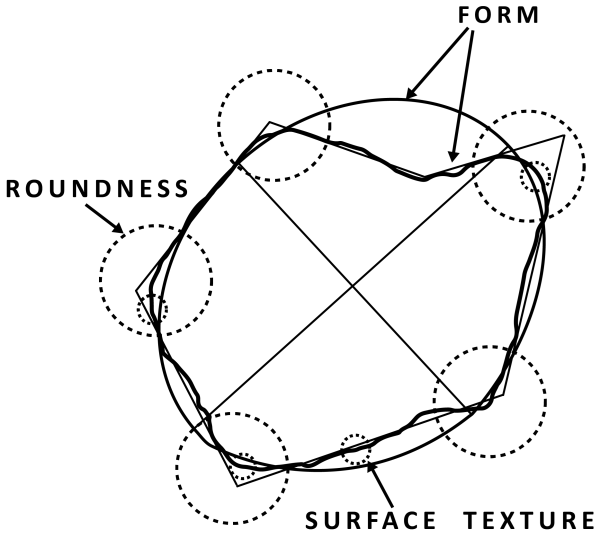
\includegraphics[scale=0.4]{fig1.png}}
\caption{Forma general, redondez y textura superficial propuestas por Barret.}
\label{fig1}
\end{figure}

La forma es un parámetro simple y existen diversas expresiones para medir la forma, una de las más usadas en el campo geológico es la propuesta por Wadell \cite{b7}, la cual se obtiene de la relación entre el radio del círculo cuya área es igual a la de la partícula y el radio del círculo más pequeño que inscribe a la partícula. Sin embargo la redondez es un parámetro difícil de estimar y por esta razón dedicamos el presente trabajo a su estimación. Para medir el grado de redondez, existen dos enfoques; los basados en curvatura \cite{b8} y los que emplean Fourier \cite{b9}. El método basado en curvatura define el grado de redondez como la relación entre el radio de curvatura promedio de las esquinas de una partícula y el radio del círculo circunscrito más grande posible.  Este método es simple y preciso, sin embargo es un método cuyos parámetros depende de la escala. Los métodos basados en Fourier son invariantes a la escala, rotación y traslación sin embargo analizar el espectro es tema complicado y de un alto costo computacional \cite{b9}.

En el presente trabajo nos planteamos usar redes neuronales para estimar la redondez de rocas sedimentarias. La variable de entrada a la red neuronal es el PCA del espectro de Fourier elíptico. Se eligió esta variable por ser invariante a la escala, la rotación y traslación.  Como objetivo de la red neuronal se empleó el grado de angulosidad calculado con el método de curvatura propuesto por Wadell \cite{b7}. Para calcular la angulosidad utilizamos el algoritmo propuesto por Zheng \cite{b8}. La red neuronal utilizada tiene la siguiente arquitectura: red  neuronal de 6 capas, la capa de entrada con 40 neuronas y función de activación ReLU, 4 capas ocultas con 40 neuronas cada una, con función de activación ReLU. La capa de salida con una sola neurona con función de activación lineal. La base de datos para entrenar la red neuronal se compone de 1125 imágenes de rocas reales de diversos fenómenos geológicos. La red neuronal tiene un error cuadrático medio de 0.029 y un error promedio de 0.017. La red neuronal nos permite tener la redondez y la circularidad en tiempo 2800 veces más rápido que el método de Wadell \cite{b7}, además de ser invariante a la escala, rotación y traslación. A través de la red neuronal hemos combinado las potencialidades del método basado en curvatura y análisis frecuencial. 




\section{Materiales y métodos}
En esta sección describiremos a detalle la definición y las expresiones matemáticas para estimar la redondez. También se describe Fourier elíptico el cual utilizamos como variable de entrada de la red neuronal. 

%\subsection{Forma general}
%La forma general, como mencionamos anteriormente, es la característica morfológica de mayor jerarquía. La forma general son variaciones en el contorno cuya magnitud esta en el misma orden del tamaño de la partícula. La forma general puede ser medida por su grado de circularidad, es decir, el grado de similitud entre la partícula y un circulo. Esta métrica,propuesta por Wadell \cite{b7}, es la más usadas en la práctica geológica y su expresión es la siguiente 
%
%\begin{equation}
%C_{D} = \frac{d_{c}}{D_{cir}} \label{eq1}
%\end{equation}
%
%donde $d_{c}$ el diámetro del círculo cuya área es igual al área de la partícula y $D_{cir}$ el diámetro del círculo más pequeño que inscribe a la partícula.


\subsection{Redondez}
La redondez es una propiedad de segundo orden que se superpone a la forma general. La redondez esta relacionada con la suavidad (o angulosidad) de la partícula. Estas variaciones se reflejan en esquinas, bordes y aristas. El grado de redondez puede ser estimado por dos enfoques: la curvatura y análisis frecuencial del contorno. El análisis frecuencial es descrito en la subsección Fourier elíptico. El primer enfoque consiste en encontrar las curvaturas más significativas en el contorno, las cuales están relacionadas con la angulosidad de la partícula. Entre más pequeño son los radios de curvatura mayor será el angulo del vértice y entre más curvaturas significativas existan más anguloso será el contorno.  En la Fig.~\ref{fig2} se muestra un ejemplo.



\begin{figure}[htbp]
\centerline{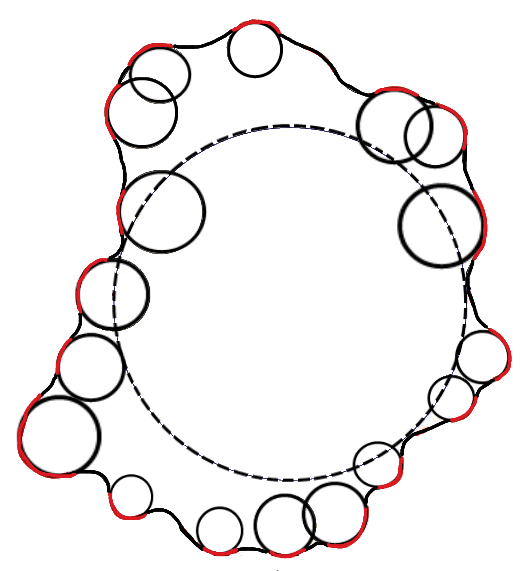
\includegraphics[scale=0.4]{fig2.png}}
\caption{Ilustración del método para medir la redondez propuesto por Wadell. Los círculos corresponden a los radios de curvatura significativos en el contorno.}
\label{fig2}
\end{figure}


Los radios de curvatura de las esquinas no pueden ser mayores al radio del máximo círculo circunscrito en la partícula, por lo que la redondez de una esquina se puede expresar como $r_{n}/R$, donde $r_{n}$ es el radio de curvatura de la esquina $n$ y $R$ es el radio del máximo círculo circunscrito. Wadell  \cite{b7} expreso la redondez total de la partícula como  

\begin{equation}
D_{g} = \sum_{n=0}^{N-1}{ \frac{r_{n}}{R}} \label{eq1}
\end{equation}

donde $N$ es número de esquinas en el contorno. De esta manera el rango de redondez esta entre 0 y 1, siendo 0 un circulo perfecto y 1 un contorno con el máximo de esquinas posibles. 

El concepto es claro, sin embargo el algoritmo para estimar esta redondez no es fácil de desarrollar.  Zheng desarrollo un algoritmo para estimar la redondez bajo este enfoque \cite{b7}. Sin embargo los parámetros dependen de la escala y el grado de redondez puede tener un alta varianza. 


\subsection{Fourier Elíptico}
El análisis frecuencial consiste en obtener la transformada de Fourier del contorno. En frecuencia, las tres características morfológicas se separan en rangos de frecuencia. El rango de baja frecuencia está relacionado con la forma general, el rango de frecuencia media con la redondez y la alta frecuencia con la rugosidad \cite{b9}. Sin embargo, determinar dónde se encuentran los límites entre los diferentes ordenes morfológicos no es una tarea fácil y ha sido un problema sin solución desde que se propuso por primera vez el método. Hasta la fecha, esta información se ha obtenido empíricamente y con gran incertidumbre.

Debido a que el contorno de las partículas es cerrado se utiliza Fourier elíptico. Este método fue propuesto por Kuhl el cual consiste en obtener los coeficientes de Fourier directamente del código de cadena del contorno \cite{b10}. El código de cadena aproxima el contorno por una secuencia de rectas que consisten en ocho direcciones, en la Fig.~\ref{fig3}.

\begin{figure}[htbp]
\centerline{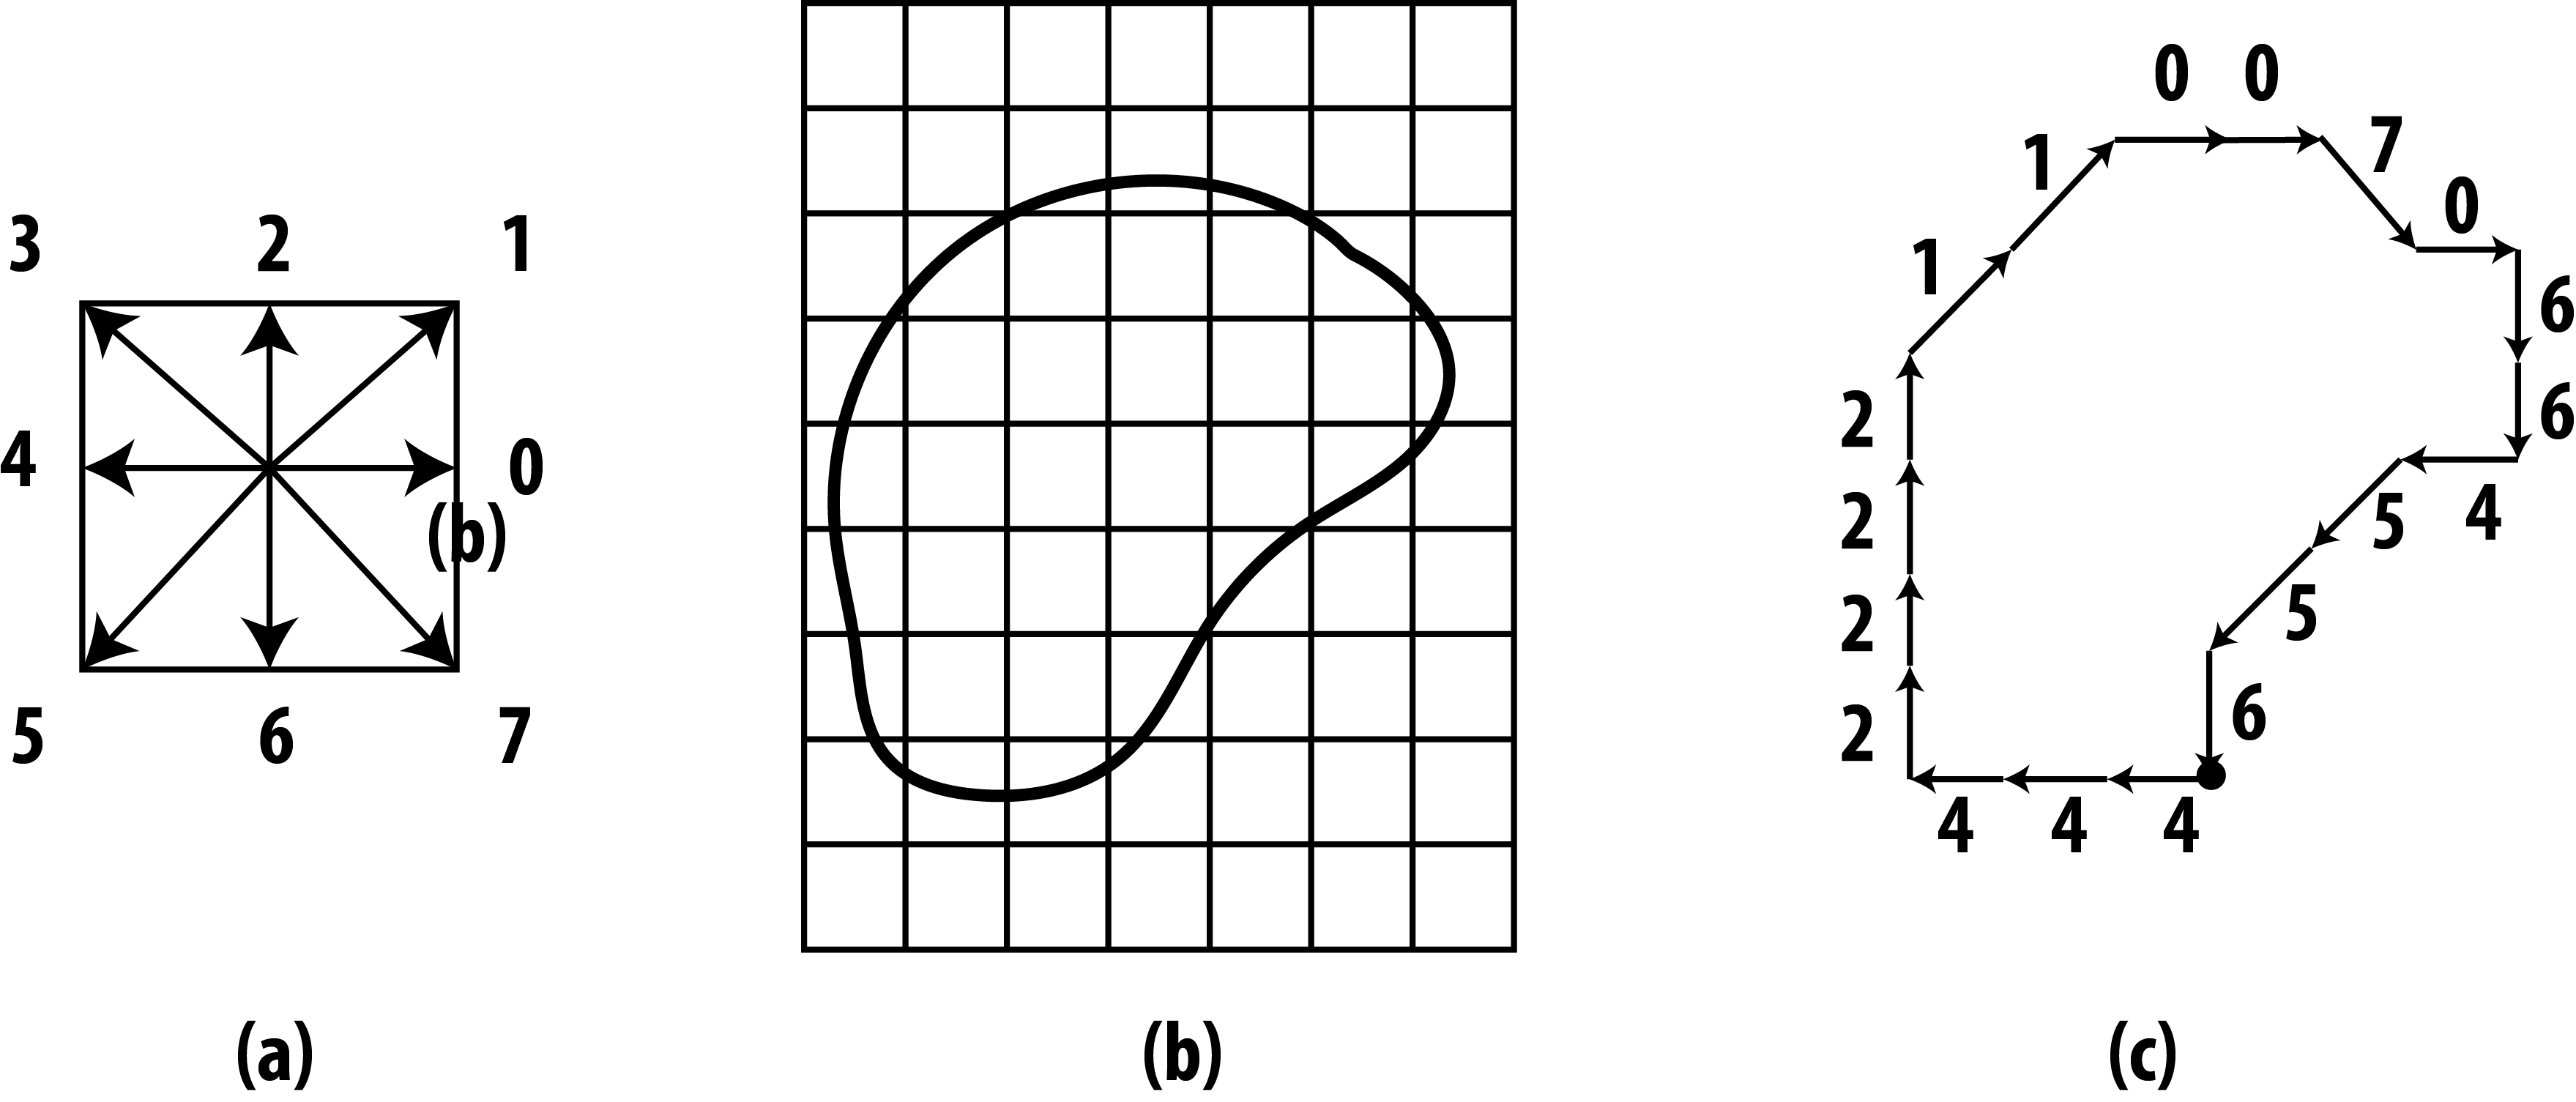
\includegraphics[scale=0.6]{fig3.png}}
\caption{Código de cadena. (a) Direcciones, (b) contorno cerrado y (c) elementos de la cadena. El punto indica el inicio de la cadena cuya resultante es 4442222110070664556.}
\label{fig3}
\end{figure}

El código de cadena puede descomponerse en dos componentes, eje $x$ y $y$, de tal manera que se pueden obtener los coeficientes por separado. Las expresiones para
los coeficientes de la componente \(x\) son

\begin{equation}
a_n = \frac{T}{2n^2\pi^2}\sum_{p = 1}^{K}\frac{\Delta x_p}{\Delta t_p}[\cos{\frac{2n\pi t_p}{T}} - \cos{\frac{2n\pi t_{p-1}}{T}}] \label{eq2}
\end{equation}

\begin{equation}
b_n = \frac{T}{2n^2\pi^2}\sum_{p = 1}^{K}\frac{\Delta x_p}{\Delta t_p}[\sin{\frac{2n\pi t_p}{T}} - \sin{\frac{2n\pi t_{p-1}}{T}}] \label{eq3}
\end{equation}

donde, la K es el número de píxeles del contorno, \(T\) el período fundamental, \(\Delta x_p\) el cambio en el eje de las x, \(\Delta t_p\) el cambio en el tiempo. De manera similar se obtienen los coeficientes de la componente \(y\) por las siguientes expresiones

\begin{equation}
c_n = \frac{T}{2n^2\pi^2}\sum_{p = 1}^{K}\frac{\Delta y_p}{\Delta t_p}[\cos{\frac{2n\pi t_p}{T}} - \cos{\frac{2n\pi t_{p-1}}{T}}] \label{eq4}
\end{equation}

\begin{equation}
d_n = \frac{T}{2n^2\pi^2}\sum_{p = 1}^{K}\frac{\Delta y_p}{\Delta t_p}[\sin{\frac{2n\pi t_p}{T}} - \sin{\frac{2n\pi t_{p-1}}{T}}] \label{eq5}
\end{equation}

Estos cuatro coeficientes pueden ser expresado mediante fasores circulares, uno para componentes, sin embargo pueden expresarse mediante un sólo fasor elíptico, de ahí proviene su nombre. Para que este método obtenga la invarianza a la escala, rotación y traslación, es necesario aplicar una normalización y ajustar el ángulo de la primer elipse en cero, las expresiones para lograr esto pueden ser consultadas en el artículo de fuente \cite{b10}. 

El resultado obtenido de Fourier elíptico son dos espectros dependientes lo que dificulta determinar los rangos de frecuencias correspondientes a la forma y redondez. 
  
\subsection{Redes neuronales profundas para determinar forma y redondez}\label{AA}
Con el fin de utilizar ambos enfoques, el de curvaturas y frecuencial, nos planteamos usar redes neuronales profundas para estimar la redondez de rocas sedimentarias. La variable de entrada a la red neuronal es el componente uno del análisis de componentes principales (ACP) del espectro de Fourier elíptico. Elegimos como variable de entrada el espectro porque este es invariante a la escala, rotación y traslación. Se aplico el ACP con el fin de reducir la dimensionalidad de los espectros resultantes de Fourier elíptico. Como objetivo, el grado de redondez obtenido mediante el método de radios de curvatura descrito anteriormente. 

Una red neuronal es un tipo de aprendizaje automático en el cual se trata de modelar el funcionamiento del cerebro humano, haciendo que la computadora pueda aprender con los casos que se van incorporando. Como su nombre lo indica, esta conformado por una cantidad de neuronas conectadas entre ellas y separadas en capas. Las conexiones son modeladas con pesos, de esta manera se le da mas o menos importancia a las conexiones entre las neuronas dependiendo de los casos del entrenamiento. Las neuronas pueden ser activadas o no mediante una función que se encarga de eso, si los pesos relacionados son positivos hace más fuerte la propagación de información, si no, más débil. Una capa esta conformada por varias neuronas y que tiene un orden específico en relación a las demás, la última capa es la que arrojará el resultado, y la primera, la que recibe los datos de entrada. Las capas que están antes de la última capa, se les denomina capas ocultas, y la última capa, se le denomina capa de salida \cite{b11}. 

\begin{figure}[htbp]
	\centerline{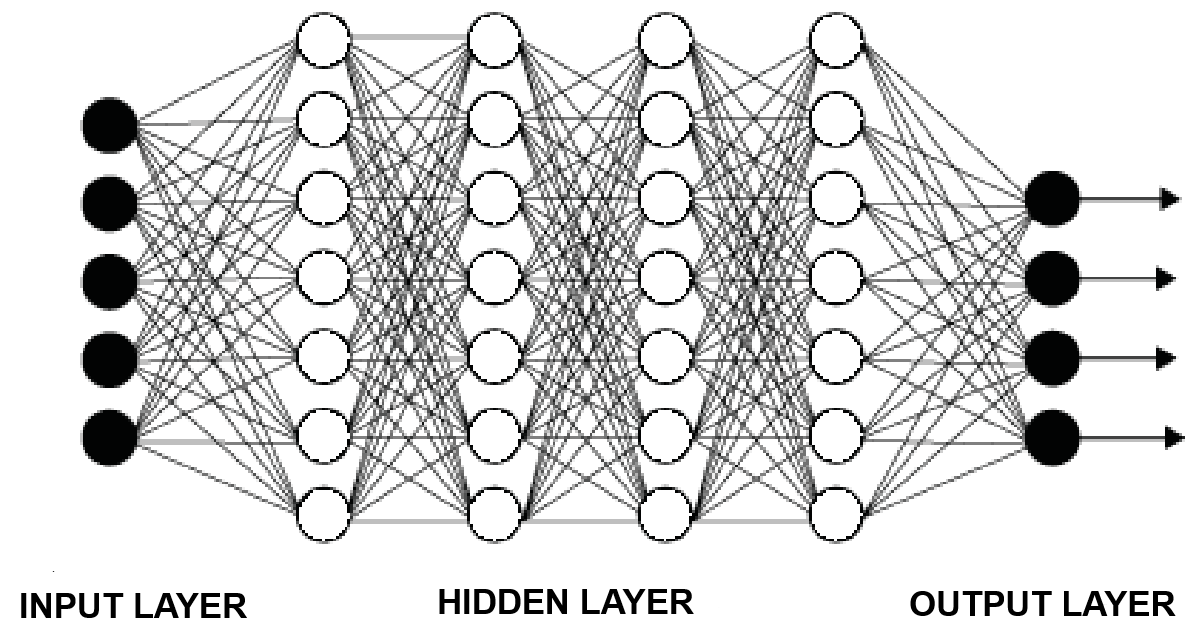
\includegraphics[scale=0.6]{fig4.png}}
	\caption{Estructura típica de una red neuronal profunda.}
	\label{fig4}
\end{figure}

Una red neuronal profunda se compone de cálculos realizados por muchas capas. En la Fig.~\ref{fig4} se puede observar una arquitectura de una red neuronal profunda con 4 capas ocultas y la capa de salida, se puede observar como se conectan los nodos de una capa con los nodos de la capa anterior y la siguiente. Este tipo de redes son utilizadas para modelar niveles de complejidad más altos y que requieren un modelo matemático más sofisticado \cite{b12}.


\section{Resultados y discusiones}
Ya hemos descrito cada una de las definiciones y expresiones que utilizamos, sin embargo, nos falta mostrar el método en su conjunto. En la Fig.~\ref{fig5} se sintetiza el flujo del método propuesto. 

\begin{figure}[htbp]
\centerline{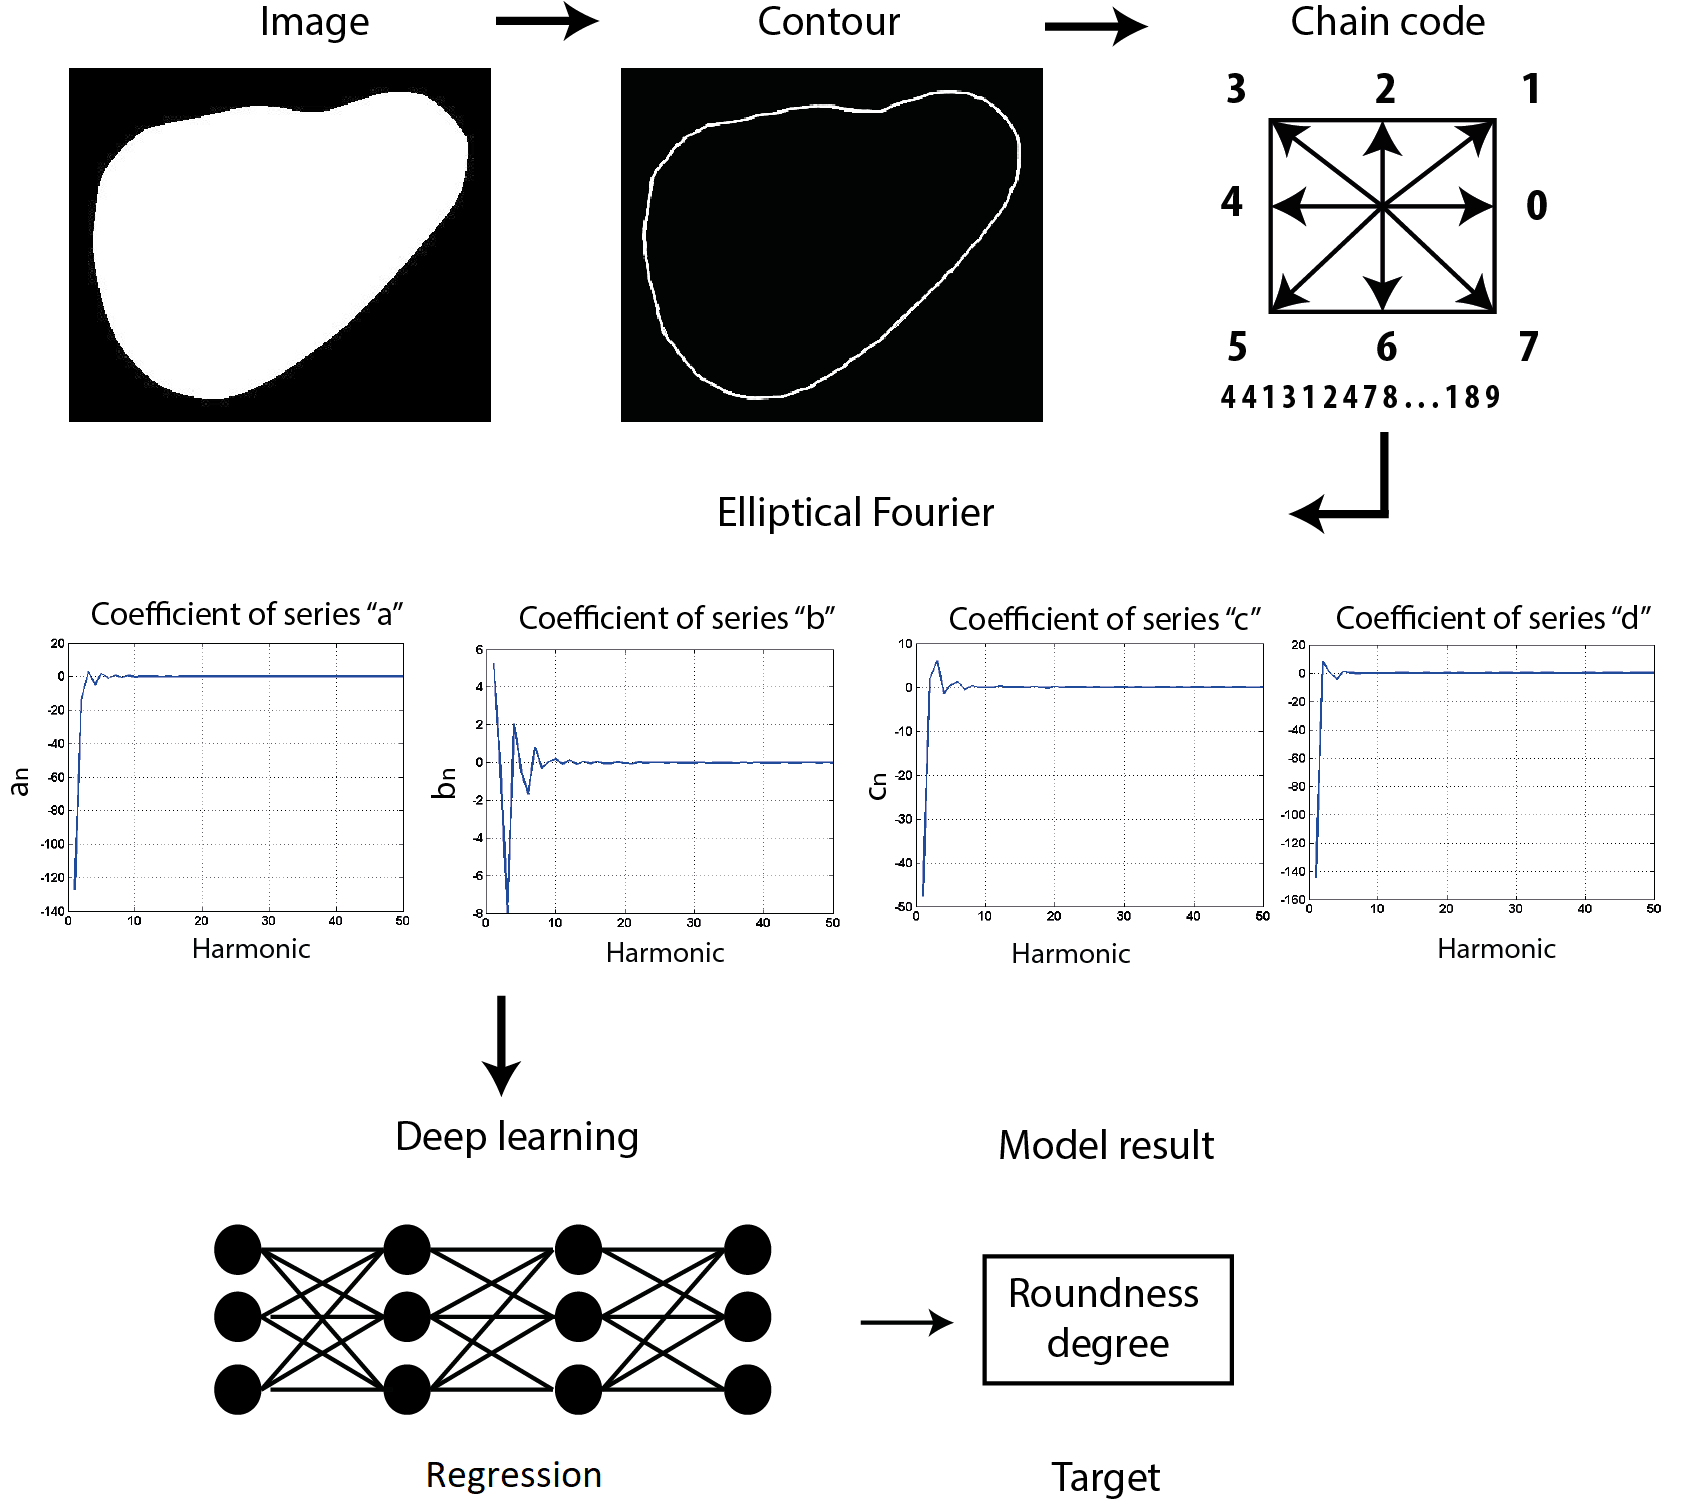
\includegraphics[scale=0.8]{fig5.png}}
\caption{Diagrama de flujo el método propuesto para medir la forma y redondez de rocas sedimentarias}
\label{fig5}
\end{figure}

La base de datos para entrenar la red neuronal se compone de 1125 imágenes de rocas reales. Las rocas analizadas son de caídas piroclásticas, flujo de bloques y cenizas, avalancha de escombros y lahares. La base de datos esta disponible en https://github.com/Gamalielmch/SedimentaryRocksImageDB. La red neuronal utilizada tiene la siguiente arquitectura: red  neuronal de 6 capas, la capa de entrada con 40 neuronas y función de activación ReLU, 4 capas ocultas con 40 neuronas cada una, con función de activación ReLU. La capa de salida con una sola neurona con función de activación lineal. La función de activación ReLU se eligió para las capas ocultas debido a que el gradiente de la función Sigmoid y la TanH puede ir desapareciendo con el avance de las épocas, esto puede afectar la propagación del error. La función de activación lineal en la capa salida es la más adecuada para nuestro propósito; problema de estimación continuo. El entrenamiento de la red neuronal fue realizado en Python v3.7.3 utilizando la plataforma Jupyter Notebook v5.7.8, usando las librerías keras y sklearn \cite{b13}. El resultado del entrenamiento es mostrado en la Fig.~\ref{fig6}

\begin{figure}[htbp]
\centerline{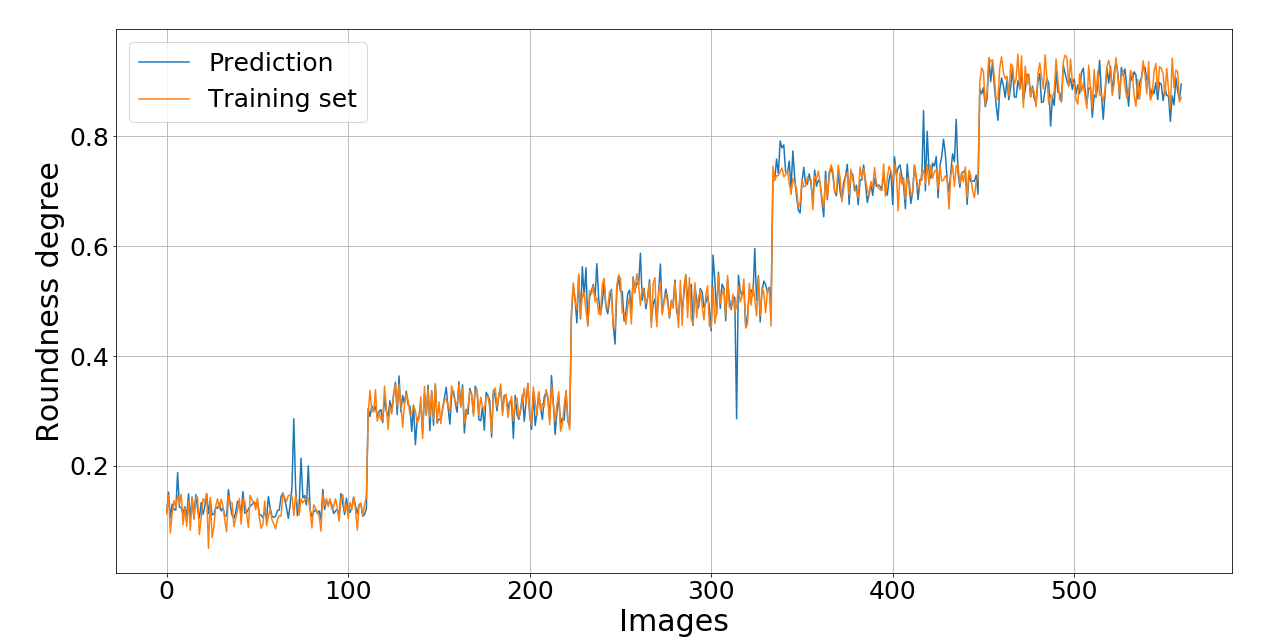
\includegraphics[scale=0.3]{fig6.png}}
\caption{Resultado del entrenamiento de red neuronal profunda}
\label{fig6}
\end{figure}

La red neuronal tiene un error cuadrático medio de 0.029 y un error promedio de 0.017. El histograma de errores de ajuste es mostrado en la Fig.~\ref{fig7}. El 91\% presentan una diferencia menor a 0.05 y el 65\% una menor a 0.02. 

\begin{figure}[htbp]
\centerline{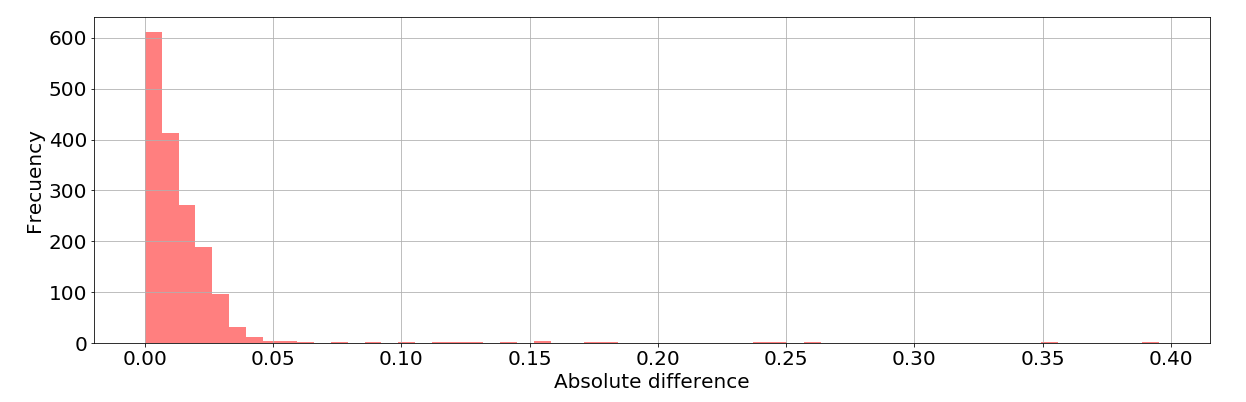
\includegraphics[scale=0.3]{fig7.png}}
\caption{Histograma de las diferencias absolutas de ajuste de la red profunda.}
\label{fig7}
\end{figure}

Para probar la red neuronal profunda hemos reservado 180 imágenes de la base de datos. En la Fig.~\ref{fig8} se muestran los resultados de estas imágenes. El error medio cuadrático es de 0.0011 y el error promedio de 0.019.

El ajuste de la red neuronal lo podemos considerar como preciso para el 91\% de los casos, ya que una diferencia menor a 0.05 es muy aceptable en estudios geológicos. Además el error medio de la imágenes de prueba confirman un buen ajuste. 

\begin{figure}[htbp]
\centerline{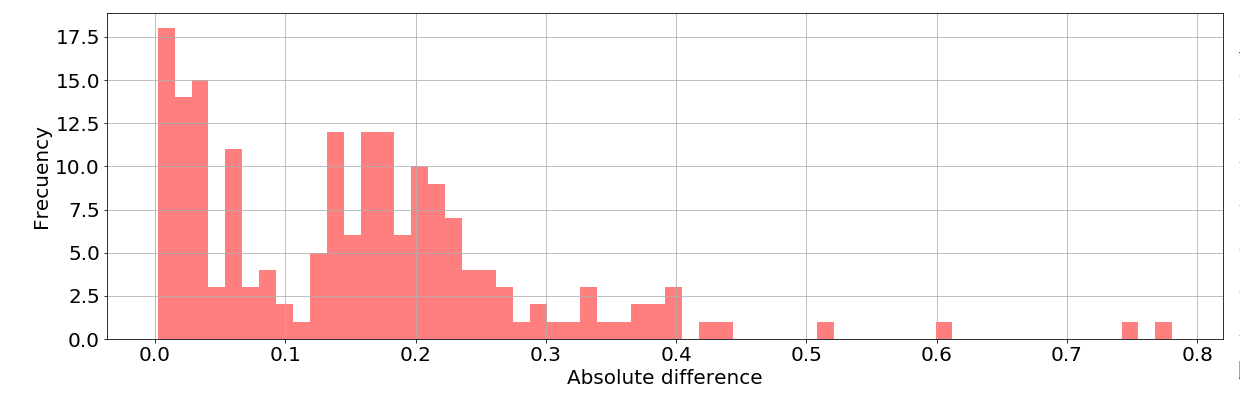
\includegraphics[scale=0.3]{fig8.png}}
\caption{Resultado de al red neuronal profunda de las imágenes de prueba}
\label{fig8}
\end{figure}

\section{Conclusiones}
Hemos estrenado una red neuronal profunda para estimar la redondez de rocas sedimentarias. Utilizamos dos enfoques, la curvatura y el análisis frecuencial. Los datos de entrada son determinados por el análisis frecuencial y los datos de salida utilizan el enfoque de curvatura. Utilizando estos dos enfoques desarrollos un método invariante a la escala, la rotación y traslación. La red fue entrenada y probada utilizando 1125 imágenes de rocas reales de diversos fenómenos geológicos. El ajuste de la red muestra que el 91\% de las partículas presentan una diferencia menor a 0.05. Por otro lado, el error medio cuadrático de los datos de prueba fue de 0.0011 y el error promedio de 0.019, diferencia altamente aceptable en el campo geológico.  

% use section* for acknowledgment
\section*{Agradecimientos}

Los autores agradecen al Conacyt por la beca de retención No. 2019-000010-01NACV-00020 y el apoyo al proyecto No. ZAC-2018-05-125266. 

	
\begin{thebibliography}{plain}
\bibitem{b1} G. Eason, B. Noble, and I. N. Sneddon, ``On certain integrals of Lipschitz-Hankel type involving products of Bessel functions,'' Phil. Trans. Roy. Soc. London, vol. A247, pp. 529--551, April 1955.
\bibitem{b2} S. jr. Boggs, ``Petrology of sedimentary rocks,'' Cambridge: Cambridge University Press., vol. III, 2013.
\bibitem{b3} J. M. Rodriguez, T. Edesk{\"{a}}r and S. Knutsson, ``Particle shape quantities and measurement techniques-A review,'' Electronic Journal of Geotechnical Engineering, vol. 18a,pp.169--198, 2013.
\bibitem{b4} M. E. Tucker, ``Sedimentary petrology: an introduction to the origin of sedimentary rocks,''John Wiley \& Sons, 2009.
\bibitem{b5} M. Diepenbroek, A. Bartholom{\"{a}}, and I. Hillert, ``How round is round? A new approach to the topic  roundness by Fourier grain shape analysis,'' Sedimentology. pp. 411--422, 1992.
\bibitem{b6} P. J. Barrett, ``The shape of rock particles, a critical review,'' Sedimentology, vol. 27, pp. 291--303, 1980.
\bibitem{b7} H. Wadell, ``Volume, shape, and roundness of rock particles,'' The Journal of Geology, vol. 40, pp. 443--451, 1932.
\bibitem{b8} J. Zheng and R. D. Hryciw, ``Particle roundness and sphericity from images of assemblies by chart estimates and computer methods,'' Journal of Geotechnical and Geoenvironmental Engineering, vol. 142, pp. 1--15, 2016.
\bibitem{b9} I. Charpentier,  D. Sarocchi  and L. A. Rodriguez, ``Particle shape analysis of volcanic clast samples with the Matlab tool MORPHEO,'' Computers and Geosciences, vol. 51, pp. 172--181, 2013.
\bibitem{b10} F.P. Kuhl and C. R. Giardina, ``Elliptic Fourier features of a closed contour,'' Computer Graphics and Image Processing, vol. 18, pp. 236--258, 1982.
\bibitem{b11} W. Sha and K. L. Edwards, ``The use of artificial neural networks in materials science based research,'' Materials \& design 28.6 (2007): 1747-1752.
\bibitem{b12} M.A. Nielsen, ``Neural networks and deep learning,'' Determination Press, 2015.
\bibitem{b13} J. Moolayil. ``Learn Keras for Deep Neural Networks,'' Apress, 2019.

\end{thebibliography}

% that's all folks
\end{document}


